% silence warning
% Package 'classicthesis' together with (scrbook) will show a set of warning messages and currently not fixable . The command below will filter all warnings from package "titlesec" beginnging with "Non standard sectioning command"
\RequirePackage{silence}
\WarningFilter{titlesec}{Non standard sectioning command}
\documentclass[
% Replace twoside with oneside if you are printing your thesis on a single side of the paper, or for viewing on screen.
  oneside,
  %twoside,
  11pt, a4paper,
  footinclude=true,
  headinclude=true,
  cleardoublepage=empty
]{scrbook}
\usepackage[usenames,dvipsnames, table]{xcolor}
\usepackage[scaled]{beramono}
\usepackage[final]{pdfpages}
\usepackage{tikz}
\usepackage{graphicx}
\usepackage{dissertation}
\usepackage[T1]{fontenc}
\usepackage{fancyvrb}
\usepackage{textcomp}
%% Aesthetic spacing redefines that look nicer to me than the defaults.
\setlength{\cftbeforechapskip}{2ex}
\setlength{\cftbeforesecskip}{0.5ex}
%% Use Helvetica-Narrow Bold for Chapter entries
\renewcommand{\cftpartfont}{%
  \fontsize{12}{14}\usefont{OT1}{phv}{bc}{n}\selectfont
}
\renewcommand{\cftchapfont}{%
  \fontsize{11}{13}\usefont{OT1}{phv}{bc}{n}\selectfont
}
\renewcommand{\cftsecfont}{%
  \fontsize{10}{11}\usefont{OT1}{phv}{}{n}\selectfont
}
\renewcommand{\cftsubsecfont}{%
  \fontsize{9}{10}\usefont{OT1}{phv}{}{n}\selectfont
}
\renewcommand{\cftfigfont}{%
  \fontsize{9}{10}\usefont{OT1}{phv}{}{n}\selectfont
}
\renewcommand{\cfttabfont}{%
  \fontsize{9}{10}\usefont{OT1}{phv}{}{n}\selectfont
}
\usepackage[all]{xy}
\makeatletter
\newcommand\footnoteref[1]{\protected@xdef\@thefnmark{\ref{#1}}\@footnotemark}
\makeatother
\hypersetup{
	colorlinks=true,
	linkcolor=black
}

%------------------------------------------------------------------------------------
% Title
%------------------------------------------------------------------------------------
\titleA{Your Thesis Title}
%\titleB{Second line in title (if any)}
%\titleC{Third  line in title (if any)}
\author{Your Full Name Goes Here}
\supervisor{Your Supervisor's Name Goes Here}
\cosupervisor{Your coo-supervisor's Name Goes Here}
\date{\myear} % change to text if date is not today
%\makeglossaries  %  either use this ...
\makeindex	% ... or this

%------------------------------------------------------------------------------------
\begin{document}\fontfamily{phv}\fontseries{mc}\selectfont
%Cover page
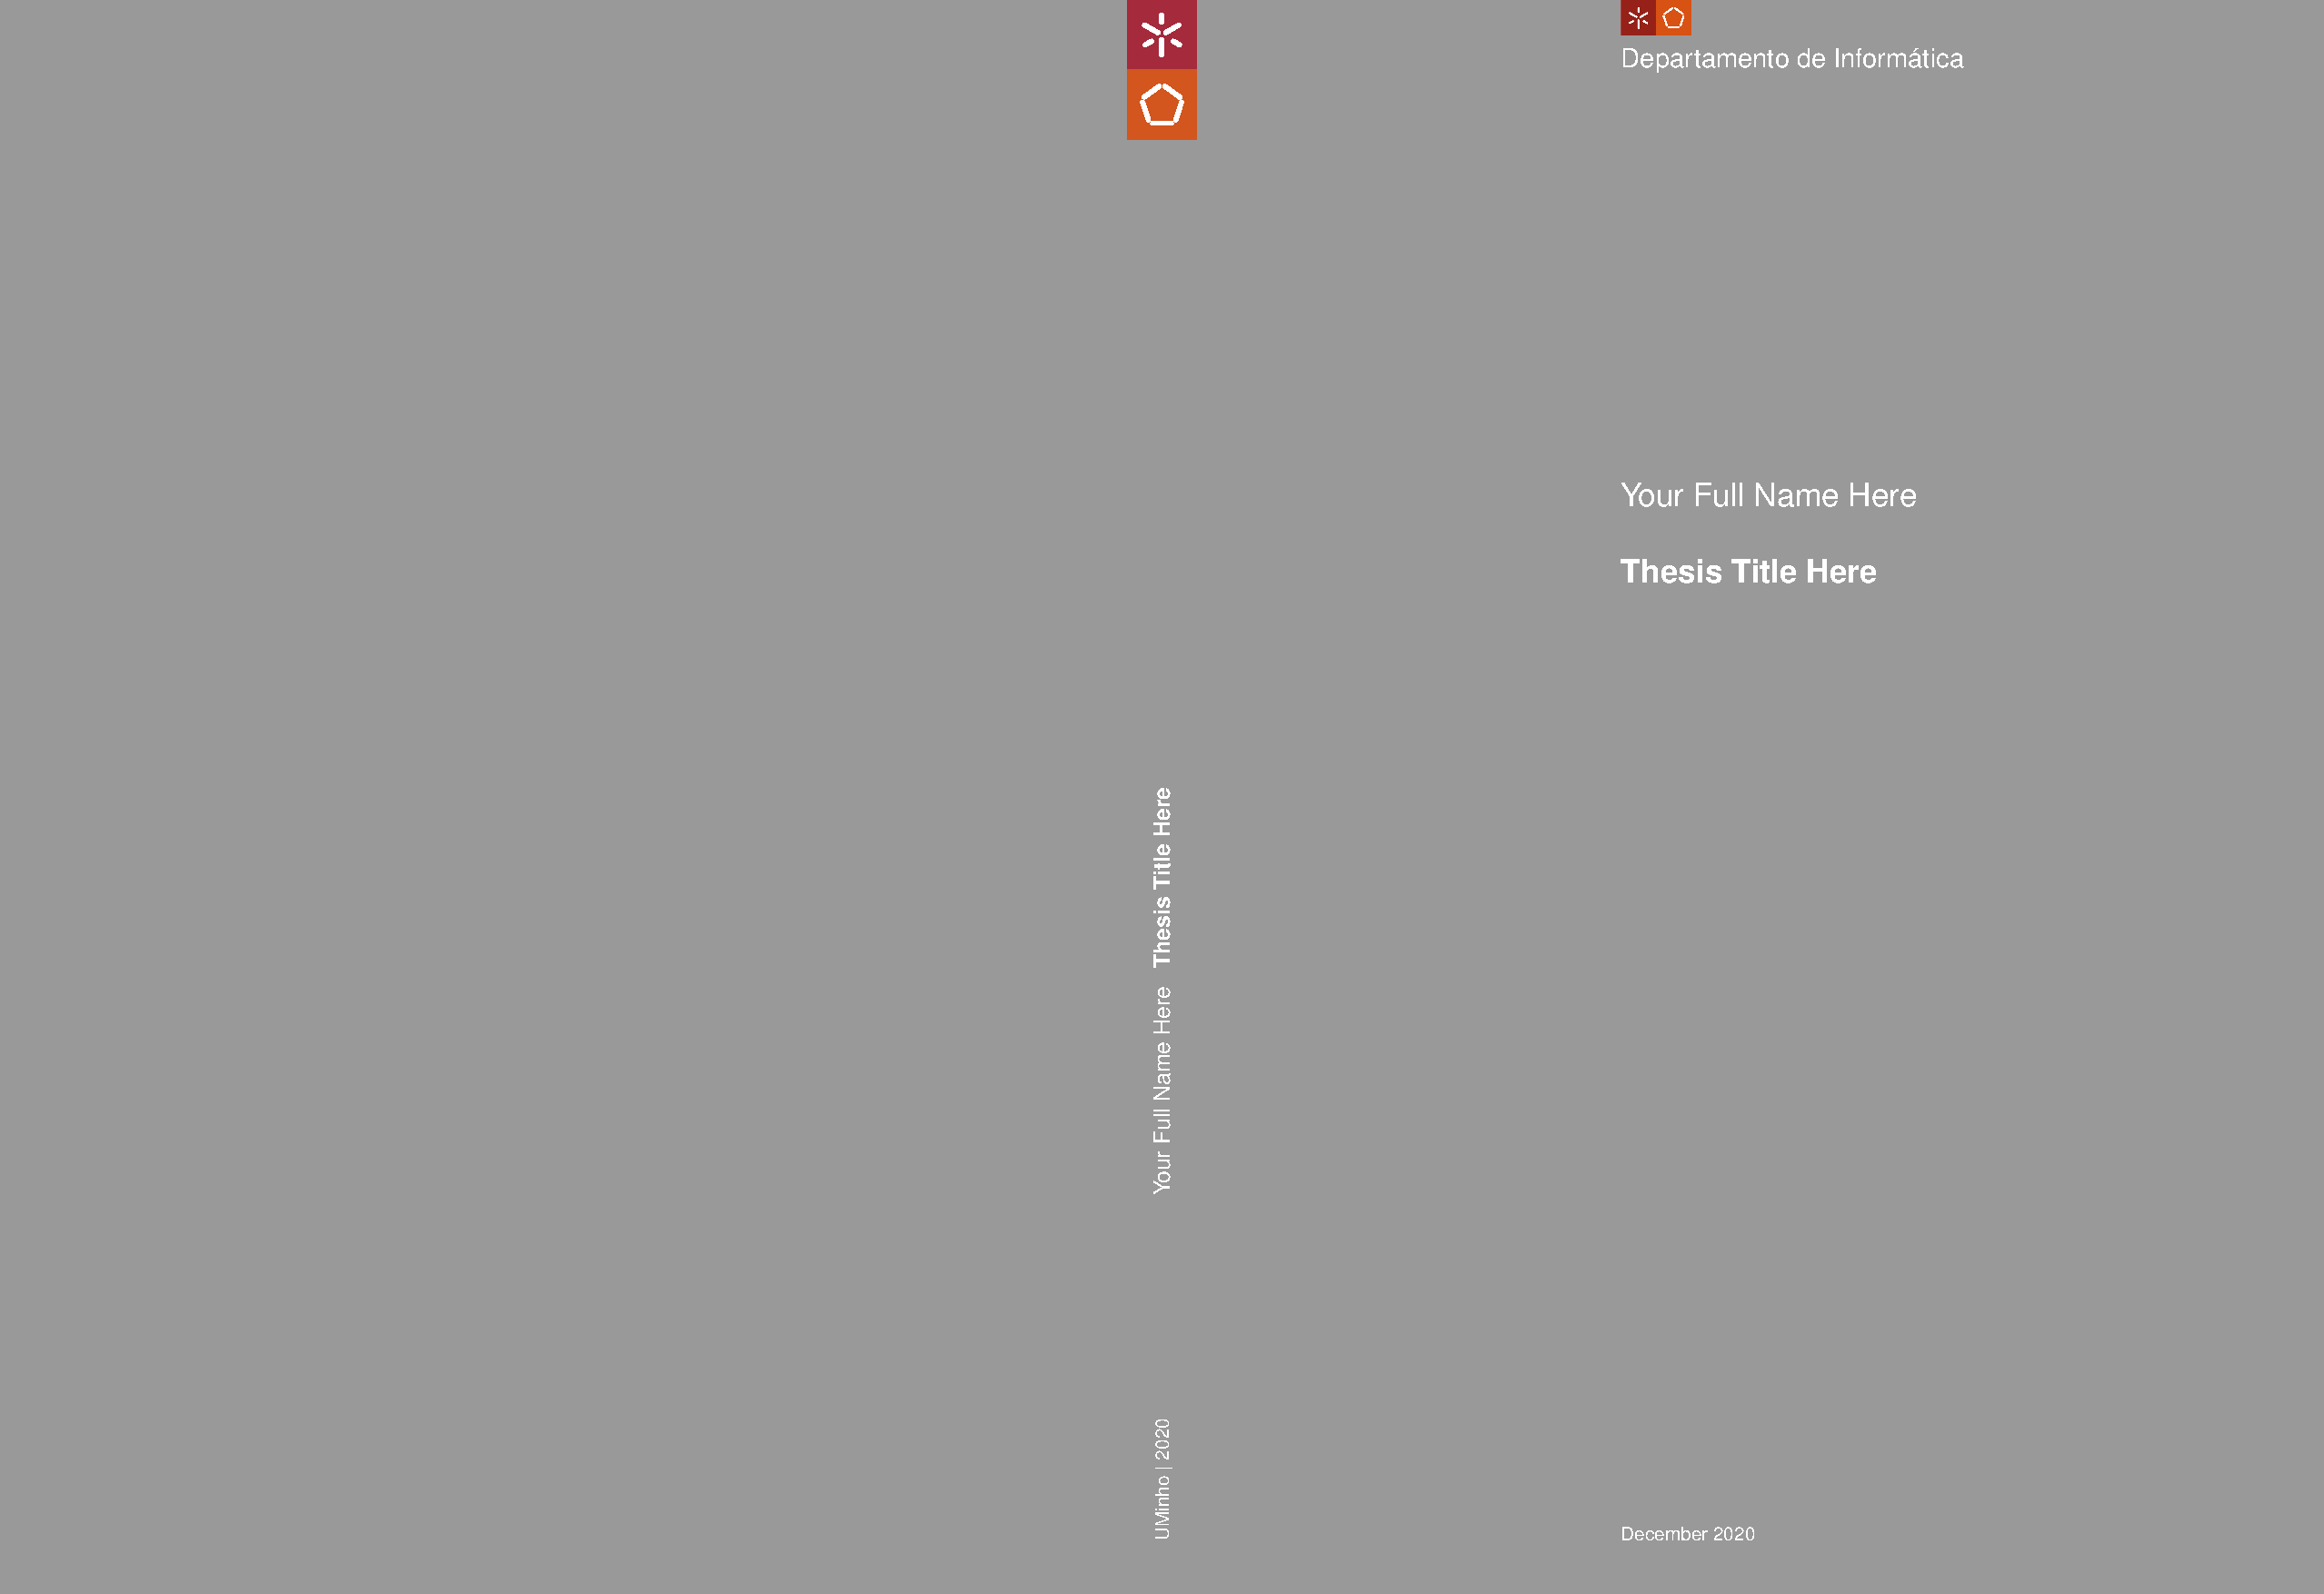
\includepdf[pages={1,2},fitpaper]{cover.pdf} 
%\thispagestyle{empty}
%!TEX root = dissertation.tex

\makeatletter

% UM_ENg Logo
\def\UMEng#1#2{\begin{tikzpicture}[
	% bars styling,
	logone/.style={rectangle,fill=white,rounded corners=0.08cm,minimum width=0.16cm,inner sep=0pt},
	bigone/.style={minimum height=0.74cm},
	smaone/.style={minimum height=0.48cm},
	engone/.style={minimum height=0.86cm},
	pos1/.style={xshift=1.3cm,yshift=1.3cm},
	pos2/.style={xshift=3.9cm,yshift=1.3cm}]
	
% Uminho logo
	\fill[fill=#1] (0,0) -- (2.6,0) -- (2.6,2.6) -- (0,2.6) -- cycle;
	\foreach \i in {1,...,3}{
		\node at (\i*120+30:0.45)[logone,bigone,pos1,rotate=\i*120-60]{};
		\node at (\i*120+90:0.60)[logone,smaone,pos1,rotate=\i*120]{};
	}

% EngUminho logo
	\fill[fill=#2] (2.6,0) -- (5.2,0) -- (5.2,2.6) -- (2.6,2.6) -- cycle;
	\foreach \i in {1,...,5}
		\node at (\i*72-90:0.74)[engone,logone,pos2,rotate=\i*72-90]{};
\end{tikzpicture}}

\def\yyy#1{\fontfamily{phv}\fontseries{mc}\selectfont {\ifnum\hide=1\relax\else#1\fi}}
\def\xxx#1{\fontfamily{phv}\fontseries{mc}\selectfont #1}
\def\zzz#1{\fontfamily{phv}\fontseries{mc}\fontseries{b}\selectfont #1}
\def\kkk#1{\fontfamily{phv}\fontseries{mc}\fontseries{b}\selectfont {\ifnum\hide=1\relax\else#1\fi}}

\long\def\coverEtc{
%Logo
~\vskip-4.1cm\rule{4cm}{0pt}\begin{tabular}{l}
\UMEng\umc{eng}
\\\zzz{Universidade do Minho}\rule{0pt}{1cm}
\\\xxx{}{Escola de Engenharia}
\\\xxx{Departamento de  Informática}
\\\rule{0pt}{4cm}
\\\xxx{{\Large\@author}}
\\\rule{0pt}{1em}
\\\zzz{\Large\@titleA}
\\\zzz{\Large\@titleB}
\\\zzz{\Large\@titleC}
\\\rule{0pt}{5cm}
\\\yyy{\large Doctoral dissertation}
%Doctor Degree in Computer Science within the Joint Doctoral Program in \\ Computer Science of the Universities of Minho, Aveiro and Porto
\\\yyy{\large Doctor Degree in Computer Science}
\\\rule{0pt}{6mm}
\\\yyy{\large Dissertation supervised by}
\\\kkk{\@supervisor}\rule{0pt}{4mm}
\\\kkk{\@cosupervisor}
\\\rule{0pt}{4.2cm}
\\\xxx{{\small\@date}}
\end{tabular}
}


\begin{frontcover}
\gdef\umc{um}\gdef\hide{1}
\thispagestyle{empty} \pagecolor{white} \textcolor{black} \coverEtc
\end{frontcover}

\begin{titlepage}
\gdef\umc{um}
\gdef\hide{0}
\thispagestyle{empty} \pagecolor{white}\textcolor{grey} \coverEtc
\end{titlepage}

\makeatother


\cleardoublepage
\pagenumbering{alph}
\setcounter{page}{0}
	
%------------------------------------------------------------------------------------
% Add Copyright and Terms of Use for Third Party Work, License, Acknowledgements, Statement of Integrity, Abstract,Resumo
\chapter*{Copyright and Terms of Use for Third Party Work}
This dissertation reports on academic work that can be used by third parties as long as the internationally accepted standards and good practices are respected concerning copyright and related rights.
\vskip 1em
\noindent This work can thereafter be used under the terms established in the license below.
\vskip 1em
\noindent Readers needing authorization conditions not provided for in the indicated licensing should contact the author through the RepositóriUM of the University of Minho.

\section*{License granted to users of this work:}

\CCBY % or replace by one in***************** the list below, cf https://alunos.uminho.pt/PT/estudantes/Formataes/3_Despacho_RT-31_2019_Anexo%203-Informa%c3%a7%c3%a3o-Direitor%20de%20Autor.docx 
%---------
%\CBYNCND
%\CCBYNCSA
%\CCBYNC
%\CCBYND
%\CCBYSA

%------------------------------------------------------------------------------------
\chapter*{Acknowledgements}
Write your acknowledgements here. Do not forget to mention the projects and grants that you have benefited from while doing your research, if any. Ask your supervisor about the specific textual format to use. (Funding agencies are quite strict about this.) 
\cleardoublepage

%------------------------------------------------------------------------------------
\chapter*{Statement of Integrity}
I hereby declare having conducted this academic work with integrity.
\vskip 1em\noindent
I confirm that I have not used plagiarism or any form of undue use of information or falsification of results along the process leading to its elaboration. 
\vskip 1em\noindent
I further declare that I have fully acknowledged the Code of Ethical Conduct of the University of Minho.
	
%------------------------------------------------------------------------------------	
% Add abstracts (en,pt) 
\chapter*{Abstract}
	Write abstract here (en) or import corresponding file

\paragraph{Keywords} keywords, here, comma, separated.

	\cleardoublepage

\chapter*{Resumo}
	Escrever aqui resumo (pt) ou importar respectivo ficheiro
	
\paragraph{Palavras-chave} palavras, chave, aqui, separadas, por, v\'{\i}rgulas



	\cleardoublepage

%------------------------------------------------------------------------------------	
\pagenumbering{roman}
\setcounter{page}{3}
%pagestyle{fancy}   % -------- removed
	
% Document
\cleardoublepage
\phantomsection
\addcontentsline{toc}{chapter}{Contents}
\tableofcontents
\cleardoublepage
\listoffigures
\cleardoublepage
\listoftables
\cleardoublepage
\lstlistoflistings
% Add list of acronyms
\cleardoublepage
\pagenumbering{arabic}
\setcounter{page}{3}


%------------------------------------------------------------------------------------
%   Chapters 
%------------------------------------------------------------------------------------
\chapter{Introduction}
\label{intro}
Write the content here...
%------------------------------------------------------------------------------------
%\bookmarksetup{startatroot} % Ends last part.
\addtocontents{toc}{\bigskip} % Making the table of contents look good.
\cleardoublepage
\bibliography{refs}
%----------------- Index of terms (needs  makeindex) --------------------------%
%\printindex
%------------------------------------------------------------------------------%
% \appendix
% \renewcommand\chaptername{Appendix}
% Add appendix chapters
\begin{backcover}
\thispagestyle{empty} \pagecolor{white} \textcolor{black} {\fontfamily{phv}\fontseries{mc}\selectfont ~\vfill
\noindent
NB: place here information about funding, FCT project, etc in which the work is framed. Leave empty otherwise.
\vfill ~}
\end{backcover}
\end{document}

